\documentclass{article}
\usepackage{amsmath}
\usepackage{amssymb}
\usepackage{algorithm}
\usepackage{float}
\usepackage{color}
\usepackage{multicol}
\usepackage{forloop}
\usepackage{graphicx}
\usepackage[margin=0.8in]{geometry}
\usepackage{caption}
\usepackage{enumerate}

\graphicspath{ {.} }
\title{MATH 3800 F\\
	\large{Assignment 3}}
\author{Krystian Wojcicki, 101001444}
\date{Winter 2020}

\begin{document}
\maketitle

\begin{enumerate}[1.]


\item \textbf{Use Simpson’s Rule with 4 subintervals to approximate $\int_{0}^{1} \frac{2}{1+x^2} dx$ to 6 decimal places.
Compare your result with the true value by calculating the simple error, ie $|true - approx|$.}

4 subintervals thus $h = \frac{1 - 0}{4} = 0.25 \Rightarrow x_0 = 0, x_1 = 0.25, x_2 = 0.5, x_3 = 0.75, x_4 = 1$

$\int_{0}^{1} \frac{2}{1+x^2} dx \simeq \frac{h}{3}[ \frac{2}{1+x_0^2} + 4\frac{2}{1+x_1^2}+ 2\frac{2}{1+x_2^2} + 4\frac{2}{1+x_3^2} + \frac{2}{1+x_4^2}]
= \frac{h}{3}[ \frac{2}{1 + 0^2} + 4\frac{2}{1+0.25^2} + 2\frac{2}{1+0.5^2} + 4\frac{2}{1+0.75^2} + \frac{2}{1+1^2}] = 1.570784$

True value of $\int_{0}^{1} \frac{2}{1+x^2} dx = 2 * \arctan(1) - 2 * \arctan(0) = 1.570796$

$Error = |true - approx| = |1.570796 -  1.570784| = 0.000012$ or $0.00076\%$

Very close to 0.

\item \textbf{Use Gaussian Quadrature with 4 steps to approximate} $\int_{0}^{1} \cos^2x dx$ \textbf{to 6 decimal places}

First change the interval from $0$ to $1 \Rightarrow -1$ to $1$.

$x = \frac{b - a}{2} * t + \frac{b + a}{2} \Rightarrow x = (1/2)t + 1/2 = (1/2)(t + 1)$ \\
$dx = 1/2 dt$

$\int_{0}^{1} \cos^2x dx = \frac{1}{2} \int_{-1}^{1} \cos^2(\frac{1}{2}(t+1)) dt \simeq \frac{1}{2}\sum_{j=1}^{4}{A_j \cos^2(\frac{1}{2}(t_j+1)} = \frac{1}{2}[
0.3478548451\cos^{2}\left(\frac{1}{2}\left(0.8611363116+1\right)\right) + 
0.3478548451\cos^{2}\left(\frac{1}{2}\left(-0.8611363116+1\right)\right) + \\
0.6521451549\cos^{2}\left(\frac{1}{2}\left(0.3399810436+1\right)\right) + 
0.6521451549\cos^{2}\left(\frac{1}{2}\left(-0.3399810436+1\right)\right)] = 0.727324318763 \simeq 0.727324
$

True value of $\int_{0}^{1} \cos^2x dx = \frac{\cos(1)\sin(1) + 1}{2} - \frac{\cos(0)\sin(0) + 0}{2} =  0.727324$

$Error = |true - approx| = 0.727324 - 0.727324 = 0$. Excellent approximation. 

\item \textbf{Use Monte Carlo simulation to approximate the probability of three tails occurring when four fair coins are flipped. Do a sufficient number of trials to have a meaningful result.}

Python 3 code: \\
\begin{center}
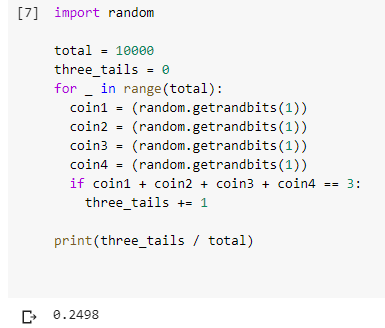
\includegraphics{a3_q3}
\end{center}

The true probability of 3 tails occurring in four fair coins is $4/16 = 0.25$ and this simulation is very close to that value.

\item \textbf{Given the loaded (unfair) dice probabilities below, use Monte Carlo simulation to simulate the results of ten rolls of the dice \\
\begin{tabular}{ c | c c c c c c}
result              & 1 & 2 & 3 & 4 & 5  & 6 \\
\hline
die 1 & 0.1 & 0.1 & 0.2 & 0.3 & 0.2 & 0.1 \\
\hline
die 2 & 0.3 & 0.1 & 0.2 & 0.1 & 0.05 & 0.25 \\
\end{tabular}
}

Python 3 code: \\
\begin{center}
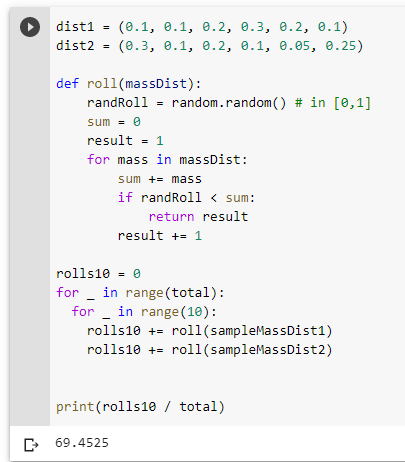
\includegraphics{a3_q4}
\end{center}

The average result of throwing each of the dies 10 times is 69.5011. 

Given the distribution table $E(x_1) = \sum_{i = 1}^{6}{P(x_1 == i) * i} = 1 * 0.1 + 2 * 0.1 + 3 * 0.2 + 4 * 0.3 + 5 * 0.2 + 6 * 0.1 = 3.7$ \\
Similarly $E(x_2) = 1 * 0.3 + 2 * 0.1 + 3 * 0.2 + 4 * 0.1 + 5 * 0.05 + 6 * 0.25 = 3.25$ \\
Meaning if 10 rolls are done the expected value is $10 * 3.7 + 10 * 3.25 = 69.5$, very close to what was found in the simulation. 

\end{enumerate}
\end{document}